\section{Gradient errors}\label{sec:2.11}

Let's turn now to the effects of gradient errors about the ideal closed orbit. These ``errors'' refer to the deviations of the focusing function $K(s)$ from its initially prescribed
- or nominal - value at each azimuth $s$. Let’s write
\begin{align}
	K(s)_{actual} = K(s)_{nominal} + \Delta K (s),
\end{align}
where we assume $\Delta K(s)$ to be a small quantity. The effect of the deviation $\Delta K(s)$ will be to change the betatron function from its nominal value $\beta(s)$ to some new value $\beta(s)+\Delta\beta(s)$. And the tune will be changed from its nominal value $\nu$ to some new value $\nu + \Delta\nu$. Generally the \emph{tune shift} $\Delta\nu$ is of more particular concern, because of the need to keep the operating point away from resonances.\\
Since the evaluation of $\Delta\beta$ is a bit tedious, I shall not give a rigorous deviation
here. I shall rather show how a simple calculation of $\Delta\nu$ can be made and then just write down the exact results for $\Delta\beta$ whose derivation can be found elsewhere\footnote{In any book on accelerators; see for example Ref. \cite{5} or \cite{7}.}.\\
Suppose that there is a gradient error $\Delta K$ in only a small azimuthal interval $\Delta s$ at $s = 0$. Then as an electron passes $s = 0$ it will receive an extra angular kick $\Delta x'$ which is proportional to its displacement $x$. In fact, by Eq.~\eqref{eq:2.19},
\begin{align}\label{eq:2.96}
	\Delta x' = \Delta K\, \Delta s\, x.
\end{align}
Let's again approximate the betatron motion by a simple harmonic oscillation; and ask what will happen when an electron arrives at $s = 0$ at the maximum of an oscillation. The motion will be as shown in Fig.~\ref{fig:fig23}. Before arriving at $s = 0$ the
\begin{figure}[!htb]
	\centering
	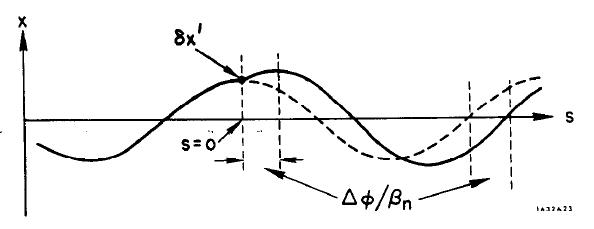
\includegraphics[width=0.8\linewidth]{./Figuras/fig23.jpeg}
	\caption{Effect of a gradient error at $s = 0$.}
	\label{fig:fig23}
\end{figure}
displacement was given by
\begin{align}
	x = b \cos{(s/\beta_n)};
\end{align}
and after $s = 0$ it will follow
\begin{align}
	x = (b + \Delta b) \cos(s/\beta_n+\Delta\varphi),
\end{align}
then
\begin{align}
	\Delta x' = -\dfrac{b+\Delta b}{\beta_n} \sin{\left(\Delta\varphi\right)}.
\end{align}
For small $\Delta x'$, $\Delta \varphi$ is small and $\Delta b$ is much less than $b$, so we can write that
\begin{align}
	\Delta \varphi \approx -\dfrac{\beta_n \Delta x'}{b}.
\end{align}
Using Eq.~\eqref{eq:2.96} for $\Delta x'$ - and remembering that at $s=0$ the displacement is $b$ - we have that
\begin{align}
	\Delta \varphi = \beta_n \Delta K \Delta s.
\end{align}
The effect of the gradient error is mainly to shift the phase of the oscillation by this $\Delta \varphi$. Now recall that the $2\pi\nu$ is just the total phase shift in one revolution; so roughly speaking the gradient error has produced
\begin{align}
	\Delta\nu \approx \dfrac{\Delta\varphi}{2\pi} = - \dfrac{\beta_n \Delta K \Delta s }{2\pi}.
\end{align}
This result is actually too large by a factor of two. The reason is that we have calculated $\Delta \varphi$ for the special case of the electron arriving at $s = 0$ at the maximum
of its oscillation. If the electron arrives at $s = 0$ with the phase $\varphi_0$, the phase
shift $\Delta\varphi$ gets reduced by the factor $\cos^2\varphi_0$ - as you can easily check.
 Since on successive turns $\varphi_0$ walks through many values we should expect the average $\Delta \varphi$ to be reduced by the average of $\cos^2\varphi_0$, which is just $1/2$. With this correction we estimate a $\Delta\nu$ which is precisely what is obtained by a more direct calculation, namely
\begin{align}
	\Delta\nu = \dfrac{1}{4\pi}\beta\, \Delta K\, \Delta s.
\end{align}

Notice that the tune shift is just proportional to the gradient error at any point and to the value of $\beta$ there. We see again that the betatron function is an indicator of the local ``sensiti-vity'' to imperfections of the guide field.\\
\begin{proof}
	Let $x = a\ \cos(\varphi-\vartheta)$ be the solution of the differential equation $x'' = -Kx$. For $K(s) = K(s)_{nominal}$, we've seen that an approximate solution exists, which is given by $x = b\ \cos(s/\beta_n + \varphi_0)$. When an electron passes $s=0$, its motion is now given by another differential equation: $x'' = -K(s)_{actual}\ x$ where $K(s)_{actual} = K(s)_{nominal} + \Delta K(s)$. This change on the focussing function $K(s)$ will lead to a variation $\Delta \beta$ on the betatron function. Both amplitude and phase depends on $\beta(s)$, so both of them will change too. These changes will be written as $\Delta b$ and $\Delta \varphi$, respectively. So, the solution for the new differential equation can be written as
	\begin{align*}
		x = (b+\Delta b)\ \cos(s/\beta_n + \varphi_0 + \Delta \varphi)
	\end{align*}
	You can notice that the term $\Delta \varphi$ is not multiplied by $s$, but the term $1/\beta_n$ is. The reason is that $\Delta \varphi$ only effects the electron motion in $s=0$, which is not the case for $s/\beta_n$.

	Now, considering the electron motion before the kick, we have that
	\begin{align*}
		x_i' &= -\frac{b}{\beta_n}\ \sin(s/\beta_n + \varphi_0)\\
		\therefore x_i'(0) &= -\frac{b}{\beta_n}\ \sin(\varphi_0)
	\end{align*}
	and after the kick,
	\begin{align*}
		x_f' = -\frac{b+\Delta b}{\beta_n}\ \sin(s/\beta_n + \Delta \varphi + \varphi_0)\\
		x_f'(0) = -\frac{b+\Delta b}{\beta_n}\ \sin(\Delta \varphi + \varphi_0)
	\end{align*}
	Then, the variation of $\Delta x'$ at $s=0$ is
	\begin{align*}
		\Delta x(0)' &= x(0)'_f - x(0)'_i\\
				  &= -\frac{b+\Delta b}{\beta_n}\ \sin(\Delta \varphi + \varphi_0) + \frac{b}{\beta_n}\ \sin(\varphi_0)
	\end{align*}
	Applying the angular transformation $\sin(\Delta \varphi + \varphi_0) = \sin(\Delta \varphi)\cos(\varphi_0) + \cos(\Delta \varphi)\sin(\varphi_0)$, it can be rewritten as
	\begin{align*}
		\Delta x' &= -\frac{b+\Delta b}{\beta_n}\ [\sin(\Delta \varphi)\cos(\varphi_0) + \cos(\Delta \varphi)\sin(\varphi_0)] + \frac{b}{\beta_n}\ \sin(\varphi_0)
	\end{align*}
	For small $\Delta x'$, $\Delta \varphi$ is small and we can approximate $\sin(\Delta \varphi) \approx \Delta \varphi$ and $\cos(\Delta \varphi) \approx 1$. We have that
	\begin{align*}
		\Delta x' &= -\frac{b+\Delta b}{\beta_n}\ [\Delta \varphi\ \cos(\varphi_0) + \sin(\varphi_0)] + \frac{b}{\beta_n}\ \sin(\varphi_0)\\
				  &= -\frac{b+\Delta b}{\beta_n}\ \Delta \varphi\ \cos(\varphi_0) - \frac{\Delta b}{\beta_n}\ \sin(\varphi_0)
	\end{align*}
	Discarding all second order terms,
	\begin{align*}
		\Delta x' &= -\frac{b}{\beta_n}\ \Delta \varphi\ \cos(\varphi_0) - \frac{\Delta b}{\beta_n}\ \sin(\varphi_0)
	\end{align*}
	Now, we know that the electron motion must be continuous. In other words, its motion right before the kick must be equal to its motion right after the kick, and we can write that
	\begin{align*}
		b\ \cos(\varphi_0) = (b+\Delta b)\ \cos(\Delta \varphi + \varphi_0)
	\end{align*}
	Applying the angular transformation $\cos(\Delta \varphi + \varphi_0) = \cos(\Delta \varphi)\cos(\varphi_0) - \sin(\Delta \varphi)\sin(\varphi_0)$ and approximating again $\sin(\Delta \varphi)$ and $\cos(\Delta \varphi)$, we have that
	\begin{align*}
		b\ \cos(\varphi_0) = (b+\Delta b)[\cos(\varphi_0)-\Delta \varphi\ \sin(\varphi_0)]
	\end{align*}
	It can be rewritten as
	\begin{align*}
		\frac{\Delta b}{(b+\Delta b)\Delta \varphi} = \tan(\varphi_0)
	\end{align*}
	Discarding all second order terms,
	\begin{align*}
		\frac{\Delta b}{b \Delta \varphi} &= \tan(\varphi_0)\\
		\therefore \Delta b &= b\ \Delta \varphi\ \tan(\varphi_0)
	\end{align*}
	Substituting this in the  $\Delta x'$ expression, we have that
	\begin{align*}
		\Delta x' &= -\frac{b}{\beta_n}\ \Delta \varphi\ \cos(\varphi_0) - \frac{b\ \Delta \varphi\ \tan(\varphi_0)}{\beta_n}\ \sin(\varphi_0)\\
				  &= -\frac{b}{\beta_n}\ \Delta \varphi\ \cos(\varphi_0) - \frac{b\ \Delta \varphi\ \sin^2(\varphi_0)}{\beta_n\ \cos(\varphi_0)}
	\end{align*}
	Multiplying both sides of the equation by $\cos(\varphi_0)$:
	\begin{align*}
		\cos(\varphi_0)\ \Delta x' &= -\frac{b}{\beta_n}\ \Delta \varphi\ \cos^2(\varphi_0) - \frac{b\ \Delta \varphi\ \sin^2(\varphi_0)}{\beta_n}\\
			&= -\frac{b\ \Delta \varphi}{\beta_n}[\cos^2(\varphi_0)+\sin^2(\varphi_0)]\\
			&= -\frac{b\ \Delta \varphi}{\beta_n}
	\end{align*}
	From \eqref{eq:2.96}, $\Delta x' = -\Delta K\ \Delta s\ x$. So,
	\begin{align*}
		-\Delta K\ \Delta s\ x\ \cos(\varphi_0) &= -\frac{b\ \Delta \varphi}{\beta_n}
	\end{align*}
	But we know that $x = b\ \cos(s/\beta_n + \varphi_0)$ and, of course, $x(0) = b\ \cos(\varphi_0)$. Substituting it in the mainly expression:
	\begin{align*}
		-\Delta K\ \Delta s\ b\ \cos^2(\varphi_0) &= -\frac{b\ \Delta \varphi}{\beta_n}\\
		\therefore \Delta \varphi &= \beta_n\ \Delta K\ \Delta s\ \cos^2(\varphi_0)
	\end{align*}
	From early discussions, we know that
	\begin{align*}
		\Delta \nu \approx \frac{\Delta \varphi}{2\pi} = \frac{\beta_n\ \Delta K\ \Delta s\ \cos^2(\varphi_0)}{2\pi}
	\end{align*}
    So, for the special case where the electron arrives at $s=0$ at the maximum of an oscillation, $\varphi_0=0$ and
    \begin{align*}
		\Delta \nu = \frac{1}{2\pi}\beta \Delta K \Delta s
	\end{align*}
    For all other cases, we can consider the average value of $\cos^2(\varphi_0)$, which is just $1/2$. So $\Delta \varphi$ is given by
	\begin{align*}
		\Delta \nu = \frac{1}{4\pi}\beta \Delta K \Delta s
	\end{align*}
\end{proof}
For a more rigorous deduction, check Section~\ref{sec:dtune_grad_err}.\\
If there is a gradient error $\Delta K(s)$ distributed around the ring, the total tune shift is
\begin{align}\label{eq:2.104}
	\Delta\nu = \dfrac{1}{4\pi}\oint \beta(s) \Delta K(s) ds.
\end{align}
I have said earlier that we might expect $\Delta\nu$ to scale as $\nu$, so that large $\nu$ -
values are to be avoided. To see that it is so, recall (from Section \ref{sec:2.10}) that $\beta$ is expected to scale roughly as $|K|^{-1/2}$. Then $\nu$ should scale as $|K|^{1/2}$. From Eq.~\eqref{eq:2.104}, $\Delta\nu$ would scale as $\Delta K\beta$ so $\Delta\nu/\nu$ would scale as $\Delta K/K$. For a given relative size of the gradient errors the tune shift $\Delta\nu$ is proportional to $\nu$. But the spacing between resonances is independent of $\nu$ so large $\nu$ values imply a more delicate machine.
A change of $\nu$ implies that there must have been a change of $\beta$ which is not evident in the simple calculation above. I shall now just write down an expression for $\Delta\beta$, and make some comments on it. It can be shown that
\begin{align}\label{eq:2.105}
	\boxed{\Delta\beta(s) = -\dfrac{\beta(s)}{2\sin{(2\pi\nu)}}\oint \Delta K(\bar{s})\beta(\bar{s})\cos{\left\lbrace 2 |\varphi(s) - \varphi(\bar{s})| + 2\pi\nu \right\rbrace} d\bar{s}},
\end{align}
where, as usual,
\begin{align*}
	\varphi(s) = \int_0^s\dfrac{d\bar{s}}{\beta(\bar{s})}.
\end{align*}
Compare this result with the one obtained in Eq.~\eqref{eq:2.94} for the closed orbit distortions. The form is similar, but with two important differences.  First, while $\beta^{1/2}$ appears in the integral for the closed orbit displacements, the first power of $\beta$ appears in the integral for $\Delta\beta$. Second, notice that the argument of the sine factor in the denominator is now $2\pi\nu$ instead of $\pi\nu$. The resonant “blow-up” of $\Delta\beta$ occurs at both integral and half integral values of $\nu$. The gradient errors introduce
 a new set of resonances in the operating diagram of $\nu_x$ versus $\nu_y$, which must be avoided in a working storage ring.
The tune shift $\Delta\nu$ comes, of course, from the change in the betatron function. From the definition of $\nu$, Eq.~\eqref{eq:2.60}, we can write that
\begin{align}
	2\pi\Delta\nu = -\oint \dfrac{\Delta\beta(s)}{\beta^2(s)}ds.
\end{align}
A straightforward integration over $s$ of $\Delta\beta/\beta^2$ using Eq.~\eqref{eq:2.105} gives the $\Delta\nu$ of Eq.~\eqref{eq:2.104}.\\
You are perhaps by now wondering about the following strange point. Although $\Delta\beta$ has a resonance blow-up at half-integral values of $\nu$, the tune shift $\Delta\nu$ does not. How can that be? The reason is that the expression we have derived for $\Delta\nu$ applies only for small changes in $\beta$, and is therefore not valid too close to a resonance, where $\Delta\beta$ diverges. A more precise calculation, which retains second order effects in the perturbation $\Delta K$, must be made to find $\Delta\nu$ - and, in fact, $\Delta\beta$ itself - near a resonance of $\nu$.
